% !TEX root = BioInspired.tex

\chapter{Slides - Heat Flow}

\section{Problem}

	Implement the heat flow diagram in the text using an insulated top and bottom layer.  

\subsection{Implementation}

	Using python and the matplotlib module, I used Dr. McGough's code from the slides to implement the diagram.  Working in the OPP lab however the computers there did not have the matplotlib installed, so I had to resort to using Python 2 rather than Python 3 which didn't appear to affect the final result much at all, if any.

\subsection{Issues}

	Like I said, the computers in the linux lab did not have matplotlib installed so Python 3 would not run the code.  Python 2 was used instead to fix this.

\subsection{Analysis}

	Aside from the Python 2, Python 3 issues, this program was very easy to implement mostly because all of the code was from the slides, except for the two if statements I added for the insulation.  Overall it turned out well and illustrated the heat flow accurately.

\begin{figure}[tbh]
\begin{center}
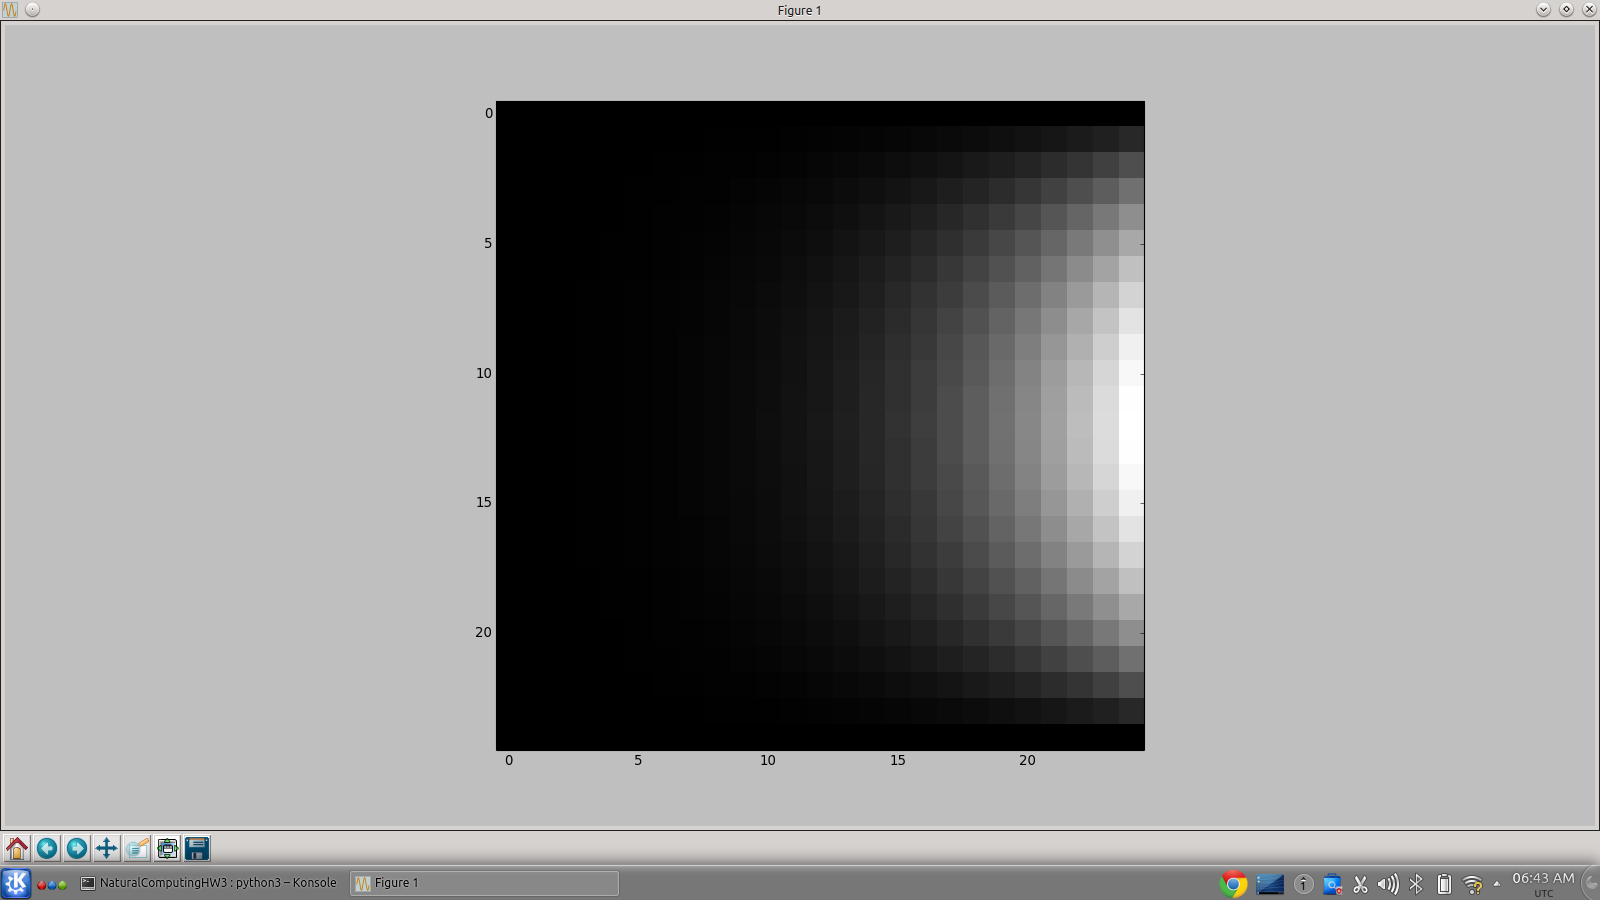
\includegraphics[width=0.75\textwidth]{heatflow.png}
\end{center}
\caption{The Heat Flow Visualization\label{fig:gprun}}
\end{figure}
